\subsection{Validation Loss}
\begin{figure}[h]
    \centering
    \begin{subfigure}[b]{0.24\textwidth}
        \centering
        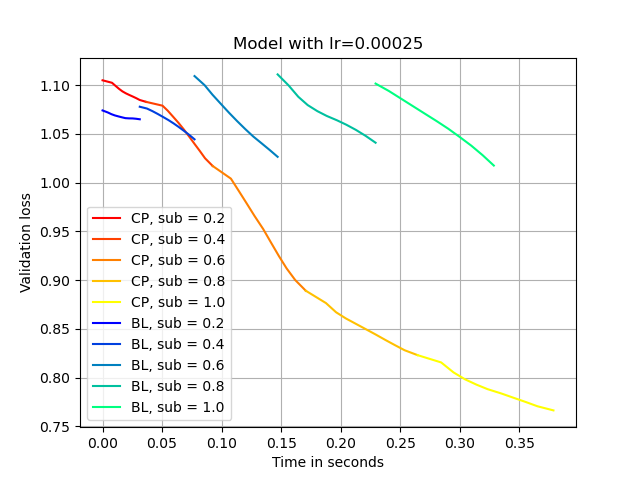
\includegraphics[width=\textwidth]{figures/22_07/iris/loss_time_0.00025.png}
        \caption{IRIS}
        \label{fig:1a}
    \end{subfigure}
    %\hfill
    \begin{subfigure}[b]{0.24\textwidth}
        \centering
        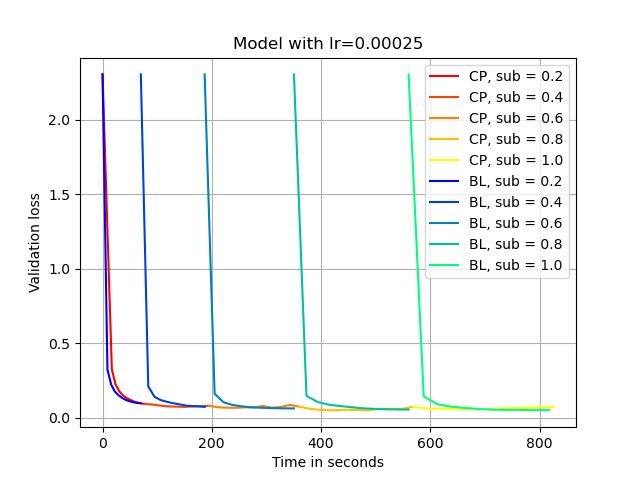
\includegraphics[width=\textwidth]{figures/22_07/10ep/loss_time_0.00025.png}
        \caption{MNIST 10 epochs}
        \label{fig:1b}
    \end{subfigure}
    %\hfill
    \begin{subfigure}[b]{0.24\textwidth}
        \centering
        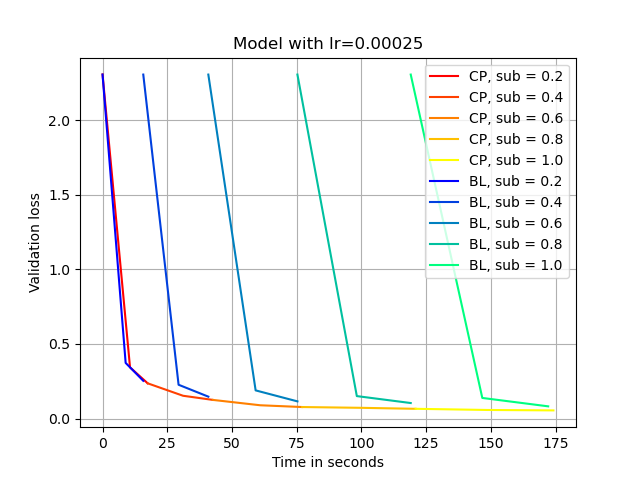
\includegraphics[width=\textwidth]{figures/22_07/2ep/loss_time_0.00025.png}
        \caption{MNIST 2 epochs}
        \label{fig:1c}
    \end{subfigure}
    %\hfill
    \begin{subfigure}[b]{0.24\textwidth}
        \centering
        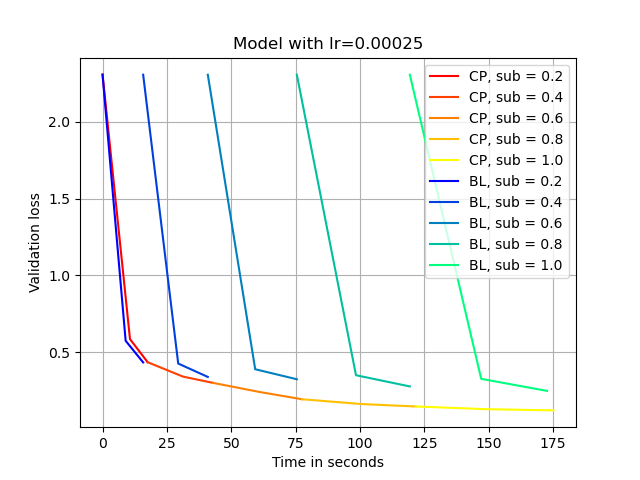
\includegraphics[width=\textwidth]{figures/22_07/2ep_smaller/loss_time_0.00025.png}
        \caption{MNIST 2 epochs, small model}
        \label{fig:1d}
    \end{subfigure}
    \caption{Visualization of validation loss versus training time for Adam optimizer and learning rate $2.5e^{-4}$}
    \label{fig:three graphs}
\end{figure}


\begin{figure}[h]
    \centering
    \begin{subfigure}[b]{0.24\textwidth}
        \centering
        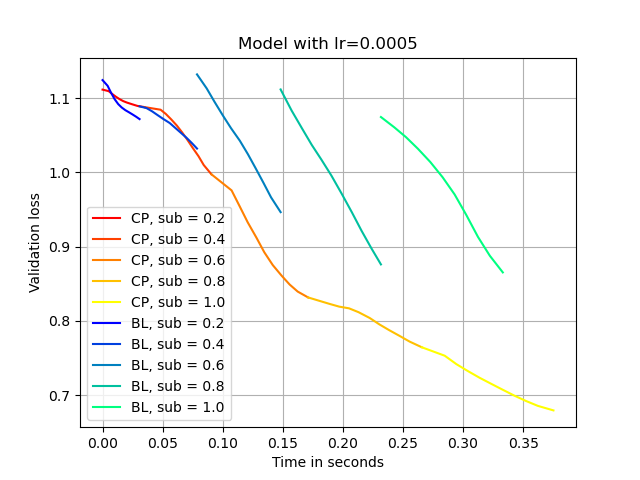
\includegraphics[width=\textwidth]{figures/22_07/iris/loss_time_0.0005.png}
        \caption{IRIS}
        \label{fig:2a}
    \end{subfigure}
    %\hfill
    \begin{subfigure}[b]{0.24\textwidth}
        \centering
        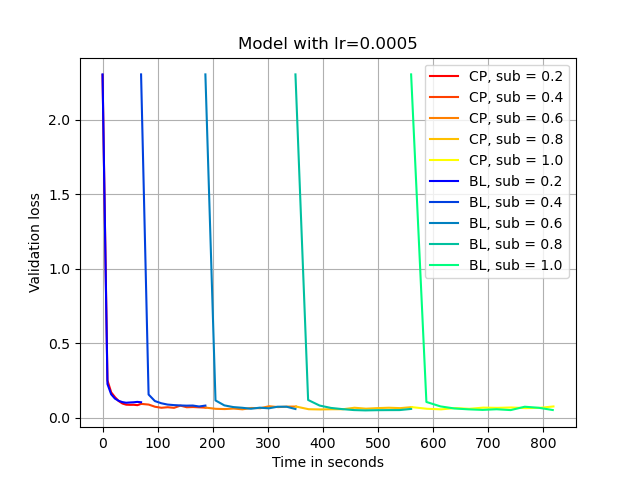
\includegraphics[width=\textwidth]{figures/22_07/10ep/loss_time_0.0005.png}
        \caption{MNIST 10 epochs}
        \label{fig:2b}
    \end{subfigure}
    %\hfill
    \begin{subfigure}[b]{0.24\textwidth}
        \centering
        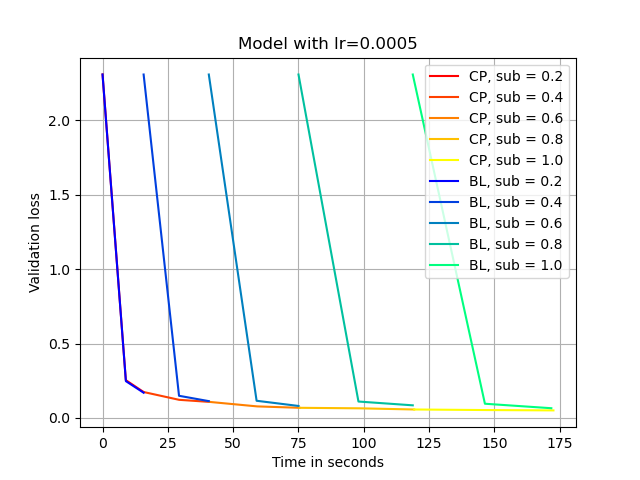
\includegraphics[width=\textwidth]{figures/22_07/2ep/loss_time_0.0005.png}
        \caption{MNIST 2 epochs}
        \label{fig:2c}
    \end{subfigure}
    %\hfill
    \begin{subfigure}[b]{0.24\textwidth}
        \centering
        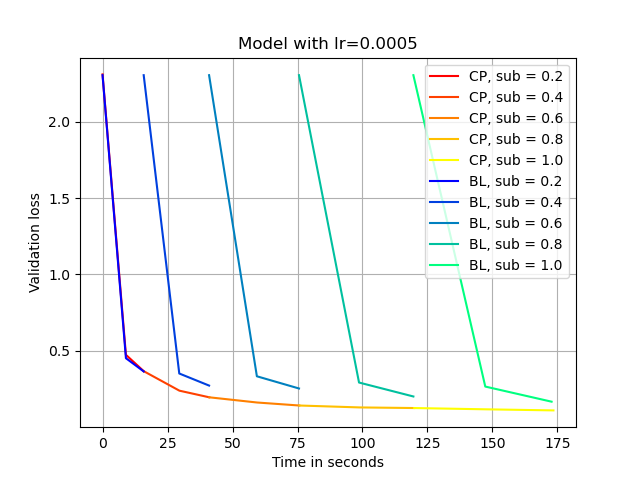
\includegraphics[width=\textwidth]{figures/22_07/2ep_smaller/loss_time_0.0005.png}
        \caption{MNIST 2 epochs, small model}
        \label{fig:2d}
    \end{subfigure}
    \caption{Visualization of validation loss versus training time for Adam optimizer and learning rate $5e^{-4}$}
    \label{fig:three graphs}
\end{figure}


\begin{figure}[h]
    \centering
    \begin{subfigure}[b]{0.24\textwidth}
        \centering
        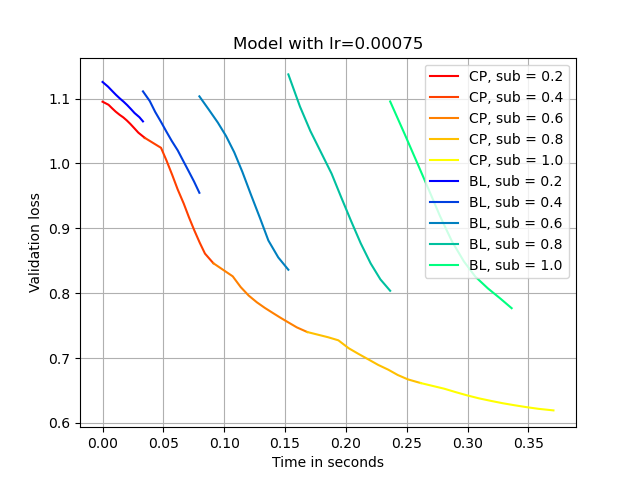
\includegraphics[width=\textwidth]{figures/22_07/iris/loss_time_0.00075.png}
        \caption{IRIS}
        \label{fig:3a}
    \end{subfigure}
    %\hfill
    \begin{subfigure}[b]{0.24\textwidth}
        \centering
        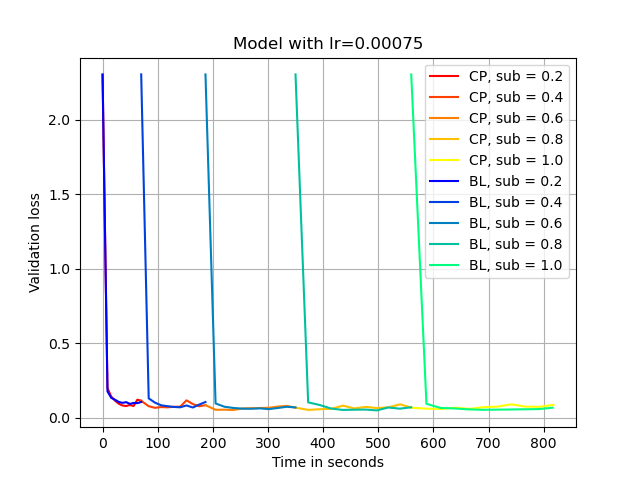
\includegraphics[width=\textwidth]{figures/22_07/10ep/loss_time_0.00075.png}
        \caption{MNIST 10 epochs}
        \label{fig:3b}
    \end{subfigure}
    %\hfill
    \begin{subfigure}[b]{0.24\textwidth}
        \centering
        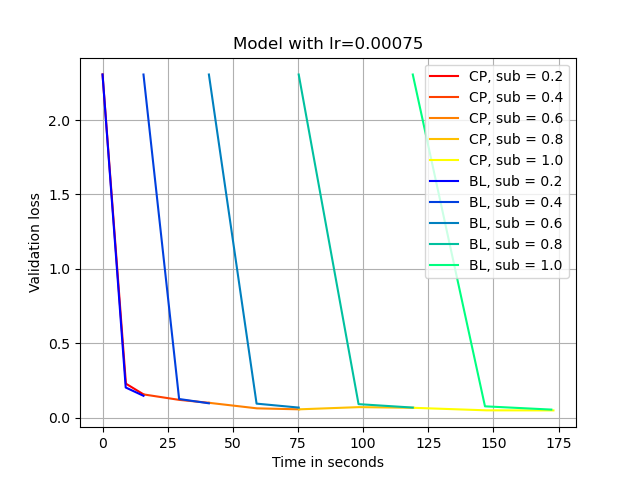
\includegraphics[width=\textwidth]{figures/22_07/2ep/loss_time_0.00075.png}
        \caption{MNIST 2 epochs}
        \label{fig:3c}
    \end{subfigure}
    %\hfill
    \begin{subfigure}[b]{0.24\textwidth}
        \centering
        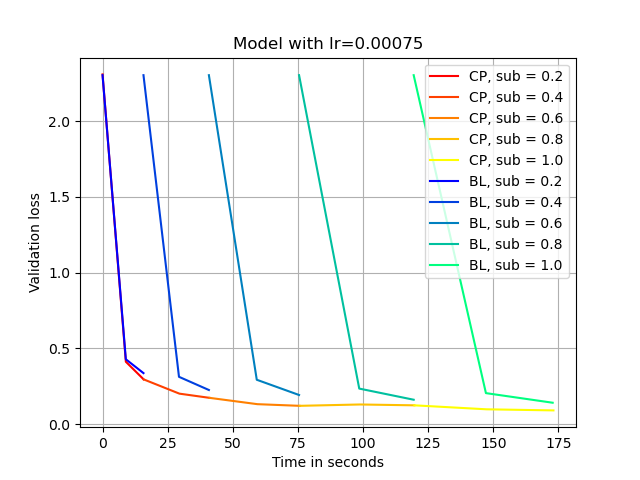
\includegraphics[width=\textwidth]{figures/22_07/2ep_smaller/loss_time_0.00075.png}
        \caption{MNIST 2 epochs, small model}
        \label{fig:3d}
    \end{subfigure}
    \caption{Visualization of validation loss versus training time for Adam optimizer and learning rate $7.5e^{-4}$}
    \label{fig:three graphs}
\end{figure}

\begin{figure}[h]
    \centering
    \begin{subfigure}[b]{0.24\textwidth}
        \centering
        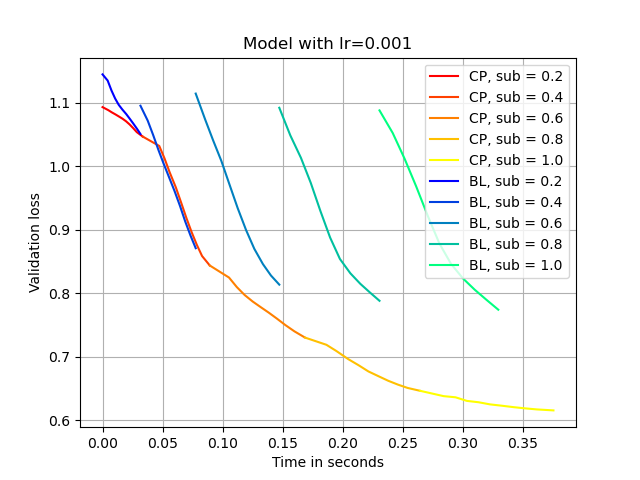
\includegraphics[width=\textwidth]{figures/22_07/iris/loss_time_0.001.png}
        \caption{IRIS}
        \label{fig:4a}
    \end{subfigure}
    %\hfill
    \begin{subfigure}[b]{0.24\textwidth}
        \centering
        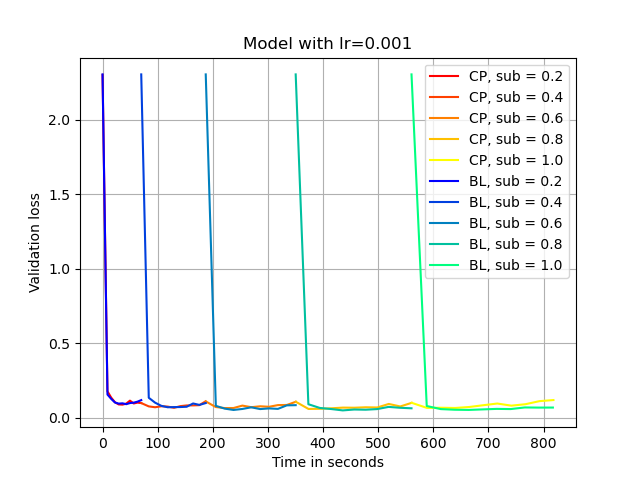
\includegraphics[width=\textwidth]{figures/22_07/10ep/loss_time_0.001.png}
        \caption{MNIST 10 epochs}
        \label{fig:4b}
    \end{subfigure}
    %\hfill
    \begin{subfigure}[b]{0.24\textwidth}
        \centering
        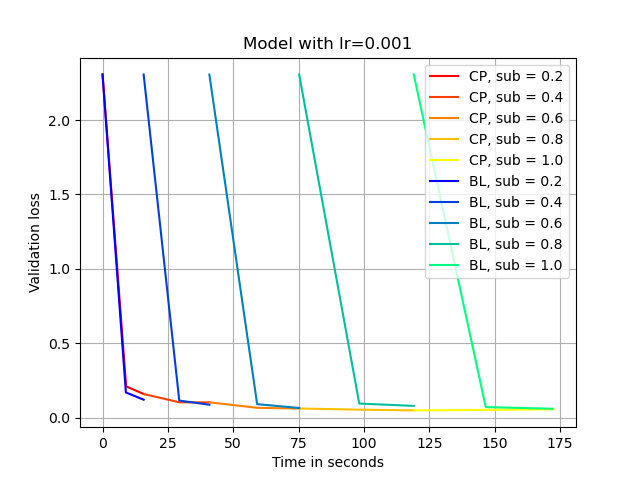
\includegraphics[width=\textwidth]{figures/22_07/2ep/loss_time_0.001.png}
        \caption{MNIST 2 epochs}
        \label{fig:4c}
    \end{subfigure}
    %\hfill
    \begin{subfigure}[b]{0.24\textwidth}
        \centering
        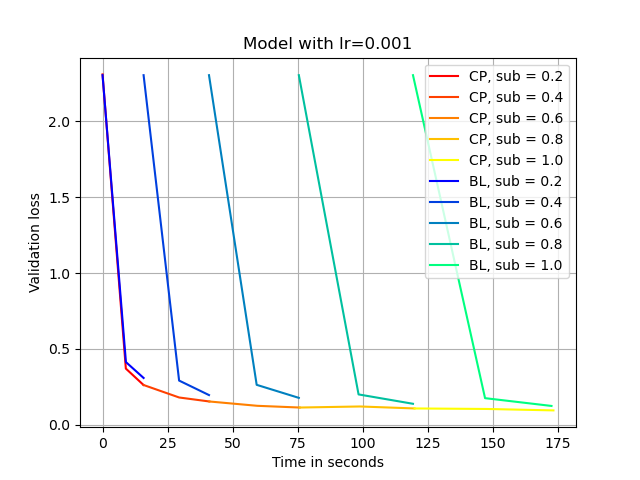
\includegraphics[width=\textwidth]{figures/22_07/2ep_smaller/loss_time_0.001.png}
        \caption{MNIST 2 epochs, small model}
        \label{fig:4d}
    \end{subfigure}
    \caption{Visualization of validation loss versus training time for Adam optimizer and learning rate $1e^{-3}$}
    \label{fig:three graphs}
\end{figure}


\begin{figure}[h]
    \centering
    \begin{subfigure}[b]{0.24\textwidth}
        \centering
        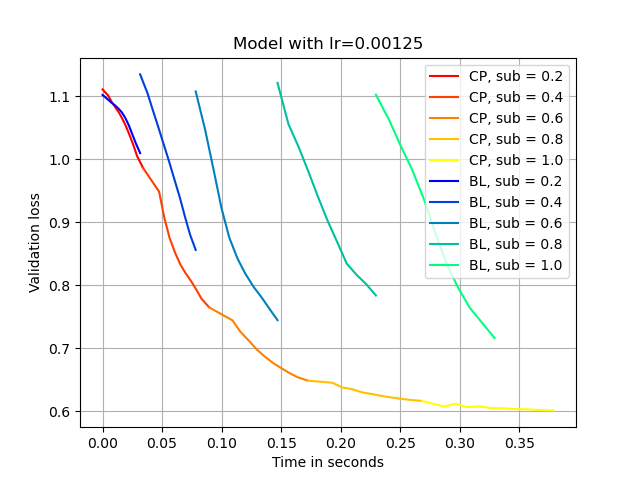
\includegraphics[width=\textwidth]{figures/22_07/iris/loss_time_0.00125.png}
        \caption{IRIS}
        \label{fig:5a}
    \end{subfigure}
    %\hfill
    \begin{subfigure}[b]{0.24\textwidth}
        \centering
        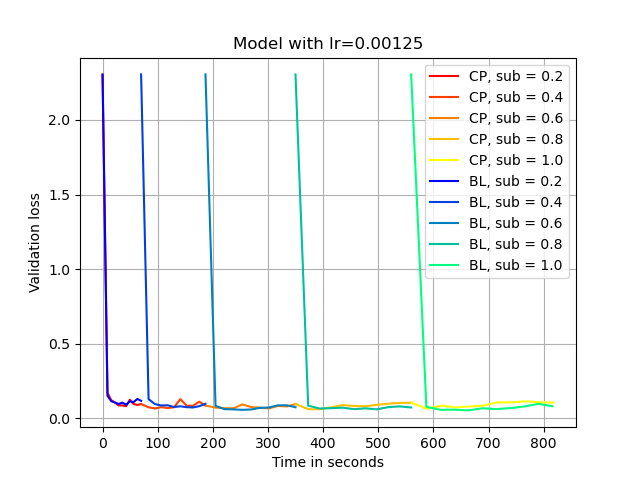
\includegraphics[width=\textwidth]{figures/22_07/10ep/loss_time_0.00125.png}
        \caption{MNIST 10 epochs}
        \label{fig:5b}
    \end{subfigure}
    %\hfill
    \begin{subfigure}[b]{0.24\textwidth}
        \centering
        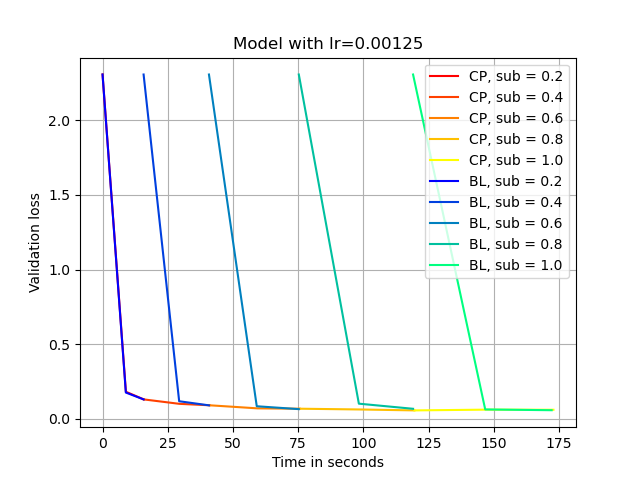
\includegraphics[width=\textwidth]{figures/22_07/2ep/loss_time_0.00125.png}
        \caption{MNIST 2 epochs}
        \label{fig:5c}
    \end{subfigure}
    %\hfill
    \begin{subfigure}[b]{0.24\textwidth}
        \centering
        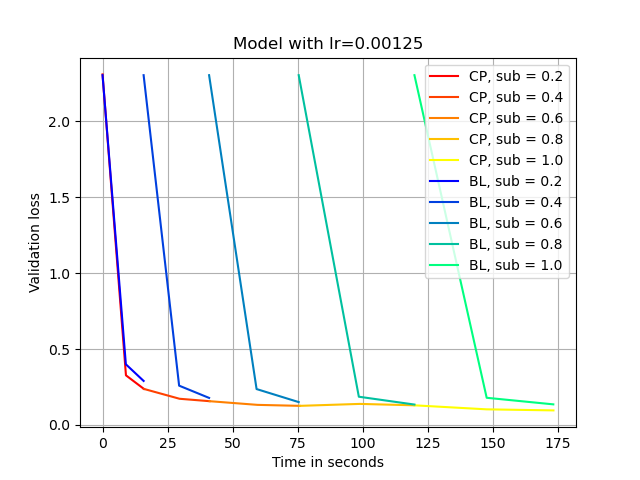
\includegraphics[width=\textwidth]{figures/22_07/2ep_smaller/loss_time_0.00125.png}
        \caption{MNIST 2 epochs, small model}
        \label{fig:5d}
    \end{subfigure}
    \caption{Visualization of validation loss versus training time for Adam optimizer and learning rate $1.25e^{-3}$}
    \label{fig:three graphs}
\end{figure}


\newpage
\subsection{Train Time}

\begin{figure}[h]
    \centering
    \begin{subfigure}[b]{0.24\textwidth}
        \centering
        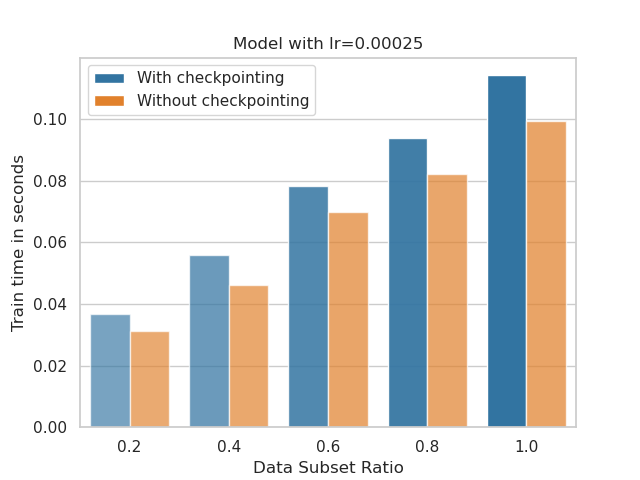
\includegraphics[width=\textwidth]{figures/22_07/iris/train_subset_0.00025.png}
        \caption{IRIS}
        \label{fig:7a}
    \end{subfigure}
    %\hfill
    \begin{subfigure}[b]{0.24\textwidth}
        \centering
        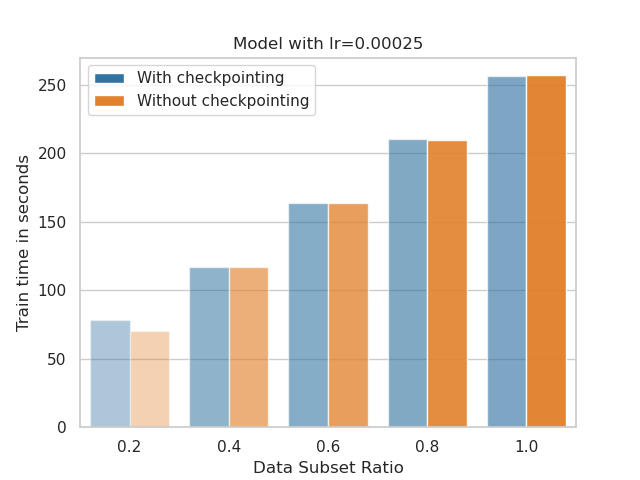
\includegraphics[width=\textwidth]{figures/22_07/10ep/train_subset_0.00025.png}
        \caption{MNIST 10 epochs}
        \label{fig:7b}
    \end{subfigure}
    %\hfill
    \begin{subfigure}[b]{0.24\textwidth}
        \centering
        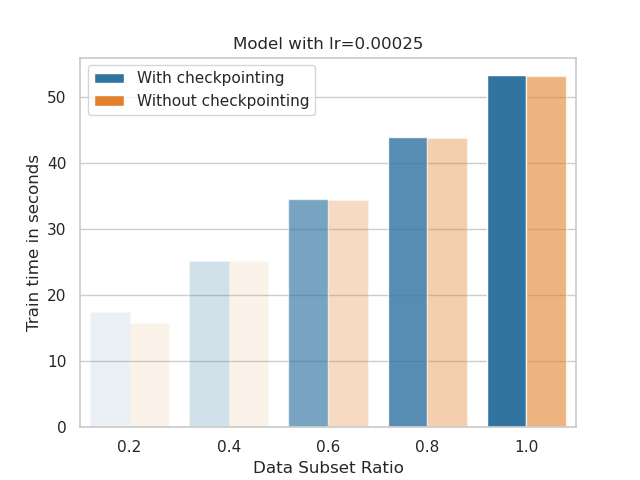
\includegraphics[width=\textwidth]{figures/22_07/2ep/train_subset_0.00025.png}
        \caption{MNIST 2 epochs}
        \label{fig:7c}
    \end{subfigure}
    %\hfill
    \begin{subfigure}[b]{0.24\textwidth}
        \centering
        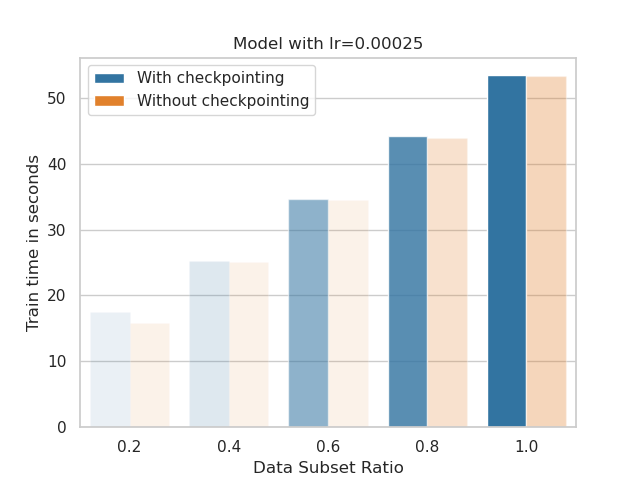
\includegraphics[width=\textwidth]{figures/22_07/2ep_smaller/train_subset_0.00025.png}
        \caption{MNIST 2 epochs, small model}
        \label{fig:7d}
    \end{subfigure}
    \caption{Visualization of the training time for every data subset ratio. A higher opacity means small validation performance difference to the optimum. An Adam optimizer and learning rate $2.5e^{-4}$ were used}
    \label{fig:7}
\end{figure}

\begin{figure}[h]
    \centering
    \begin{subfigure}[b]{0.24\textwidth}
        \centering
        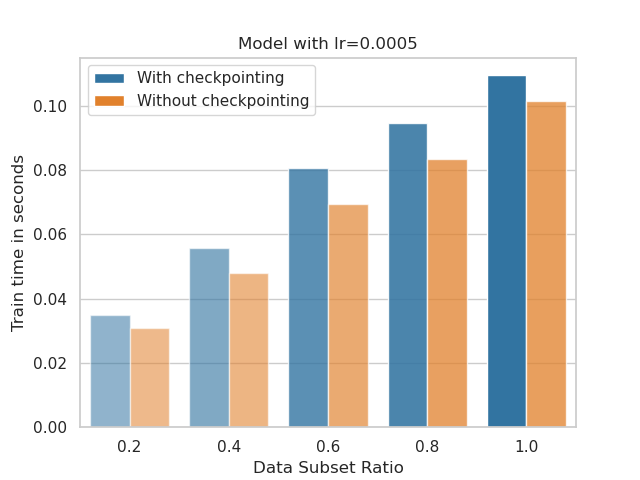
\includegraphics[width=\textwidth]{figures/22_07/iris/train_subset_0.0005.png}
        \caption{IRIS}
        \label{fig:8a}
    \end{subfigure}
    %\hfill
    \begin{subfigure}[b]{0.24\textwidth}
        \centering
        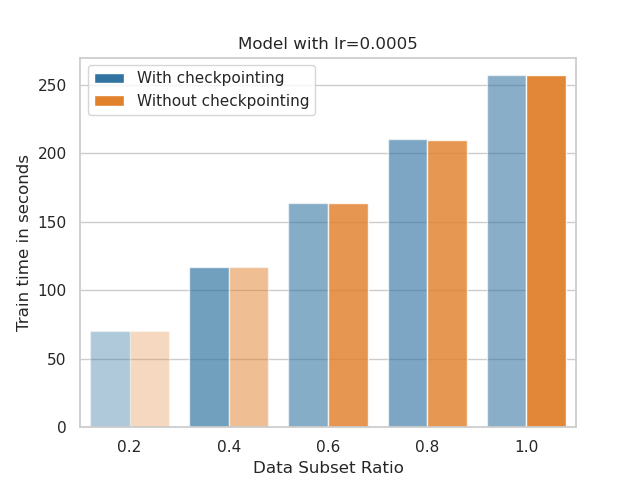
\includegraphics[width=\textwidth]{figures/22_07/10ep/train_subset_0.0005.png}
        \caption{MNIST 10 epochs}
        \label{fig:8b}
    \end{subfigure}
    %\hfill
    \begin{subfigure}[b]{0.24\textwidth}
        \centering
        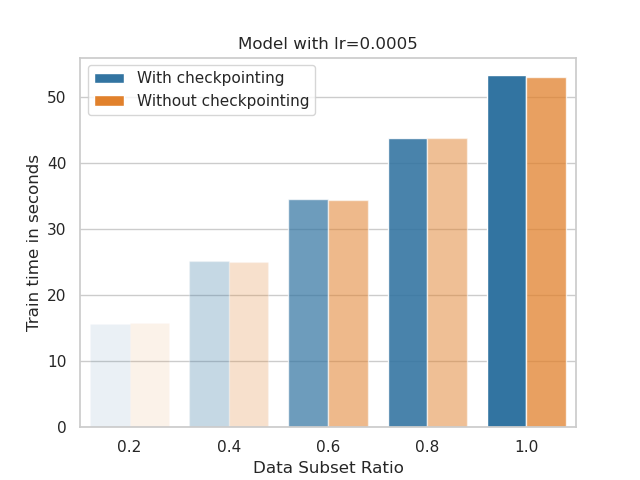
\includegraphics[width=\textwidth]{figures/22_07/2ep/train_subset_0.0005.png}
        \caption{MNIST 2 epochs}
        \label{fig:8c}
    \end{subfigure}
    %\hfill
    \begin{subfigure}[b]{0.24\textwidth}
        \centering
        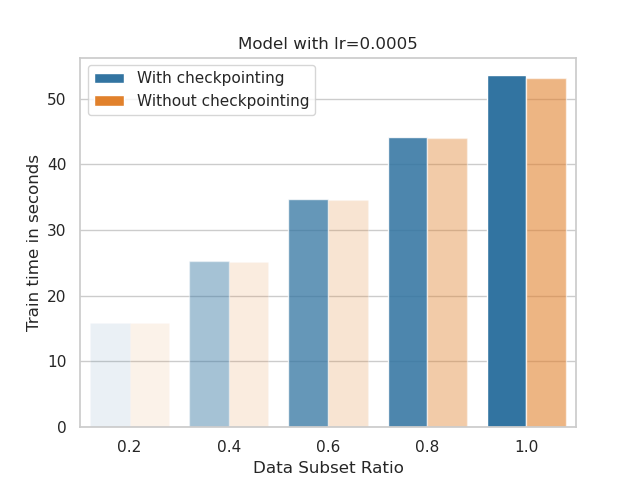
\includegraphics[width=\textwidth]{figures/22_07/2ep_smaller/train_subset_0.0005.png}
        \caption{MNIST 2 epochs, small model}
        \label{fig:8d}
    \end{subfigure}
    \caption{Visualization of the training time for every data subset ratio. A higher opacity means small validation performance difference to the optimum. An Adam optimizer and learning rate $5e^{-4}$ were used}
    \label{fig:8}
\end{figure}

\begin{figure}[h]
    \centering
    \begin{subfigure}[b]{0.24\textwidth}
        \centering
        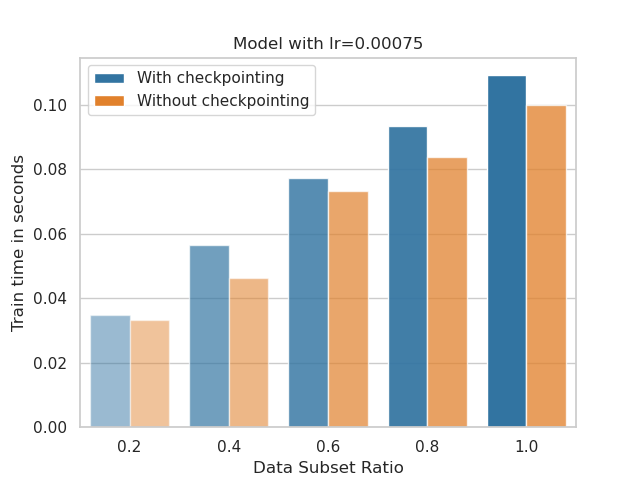
\includegraphics[width=\textwidth]{figures/22_07/iris/train_subset_0.00075.png}
        \caption{IRIS}
        \label{fig:9a}
    \end{subfigure}
    %\hfill
    \begin{subfigure}[b]{0.24\textwidth}
        \centering
        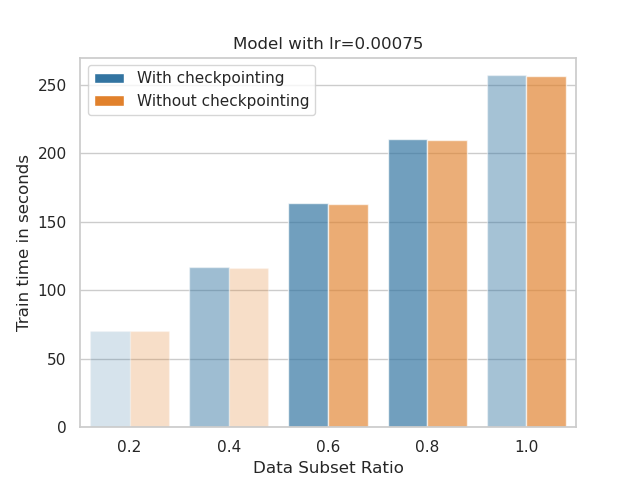
\includegraphics[width=\textwidth]{figures/22_07/10ep/train_subset_0.00075.png}
        \caption{MNIST 10 epochs}
        \label{fig:9b}
    \end{subfigure}
    %\hfill
    \begin{subfigure}[b]{0.24\textwidth}
        \centering
        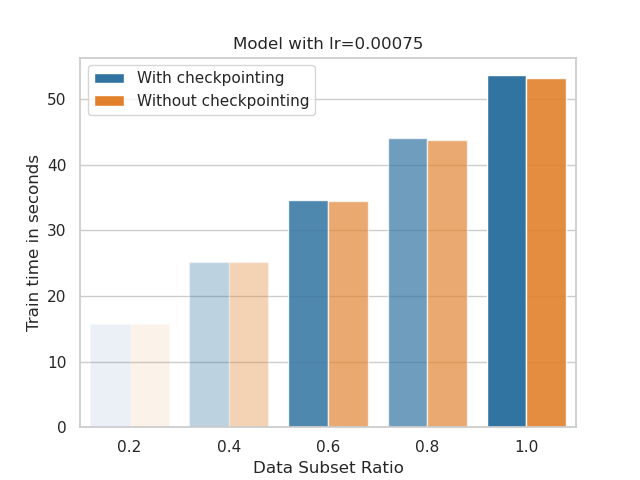
\includegraphics[width=\textwidth]{figures/22_07/2ep/train_subset_0.00075.png}
        \caption{MNIST 2 epochs}
        \label{fig:9c}
    \end{subfigure}
    %\hfill
    \begin{subfigure}[b]{0.24\textwidth}
        \centering
        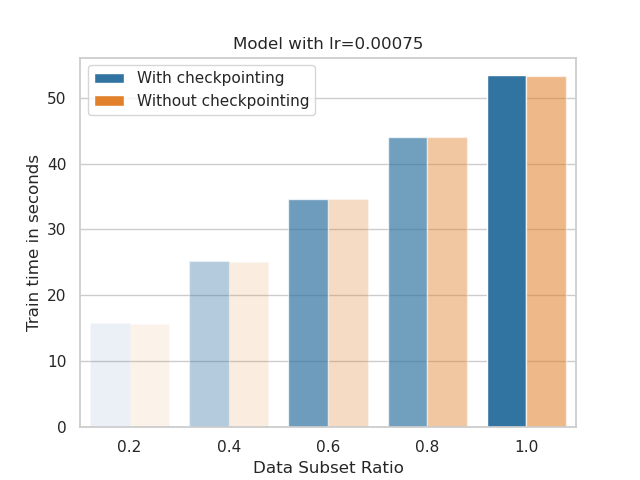
\includegraphics[width=\textwidth]{figures/22_07/2ep_smaller/train_subset_0.00075.png}
        \caption{MNIST 2 epochs, small model}
        \label{fig:9d}
    \end{subfigure}
    \caption{Visualization of the training time for every data subset ratio. A higher opacity means small validation performance difference to the optimum. An Adam optimizer and learning rate $7.5e^{-4}$ were used}
    \label{fig:9}
\end{figure}
\newpage
\begin{figure}[h]
    \centering
    \begin{subfigure}[b]{0.24\textwidth}
        \centering
        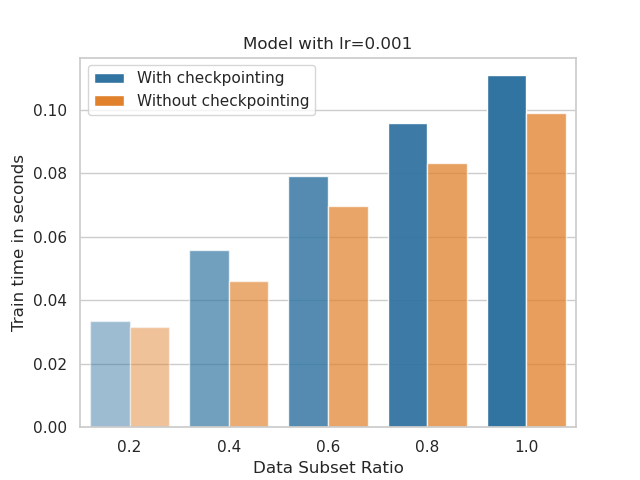
\includegraphics[width=\textwidth]{figures/22_07/iris/train_subset_0.001.png}
        \caption{IRIS}
        \label{fig:10a}
    \end{subfigure}
    %\hfill
    \begin{subfigure}[b]{0.24\textwidth}
        \centering
        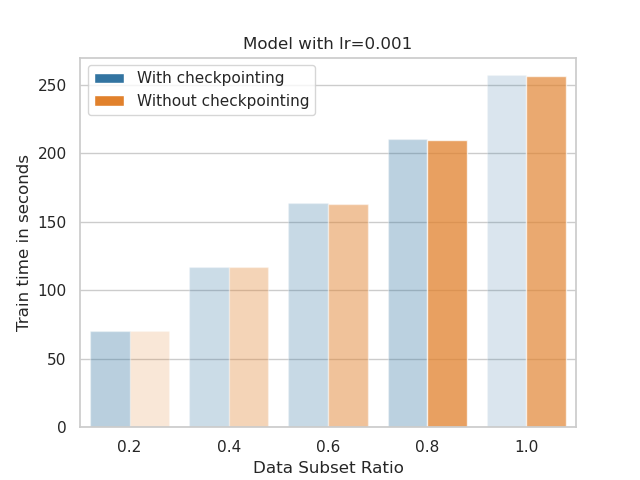
\includegraphics[width=\textwidth]{figures/22_07/10ep/train_subset_0.001.png}
        \caption{MNIST 10 epochs}
        \label{fig:10b}
    \end{subfigure}
    %\hfill
    \begin{subfigure}[b]{0.24\textwidth}
        \centering
        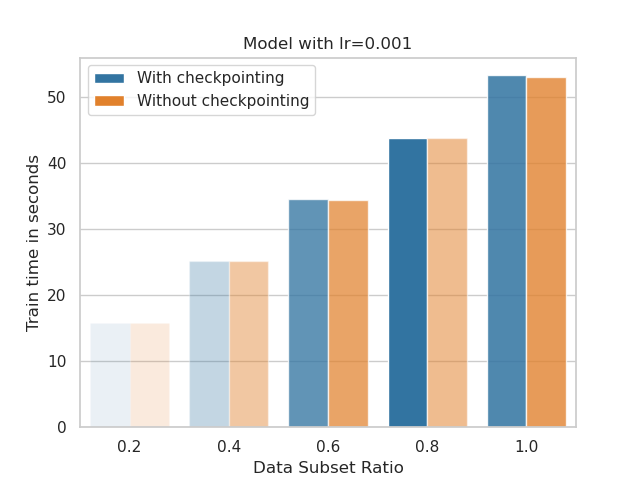
\includegraphics[width=\textwidth]{figures/22_07/2ep/train_subset_0.001.png}
        \caption{MNIST 2 epochs}
        \label{fig:10c}
    \end{subfigure}
    %\hfill
    \begin{subfigure}[b]{0.24\textwidth}
        \centering
        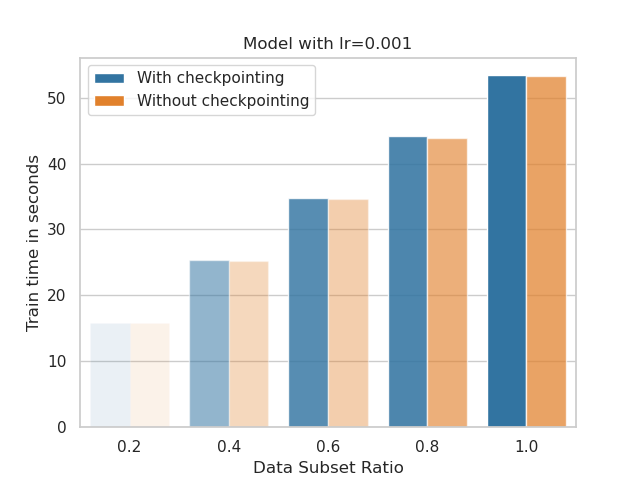
\includegraphics[width=\textwidth]{figures/22_07/2ep_smaller/train_subset_0.001.png}
        \caption{MNIST 2 epochs, small model}
        \label{fig:10d}
    \end{subfigure}
    \caption{Visualization of the training time for every data subset ratio. A higher opacity means small validation performance difference to the optimum. An Adam optimizer and learning rate $1e^{-3}$ were used}
    \label{fig:10}
\end{figure}

\begin{figure}[h]
    \centering
    \begin{subfigure}[b]{0.24\textwidth}
        \centering
        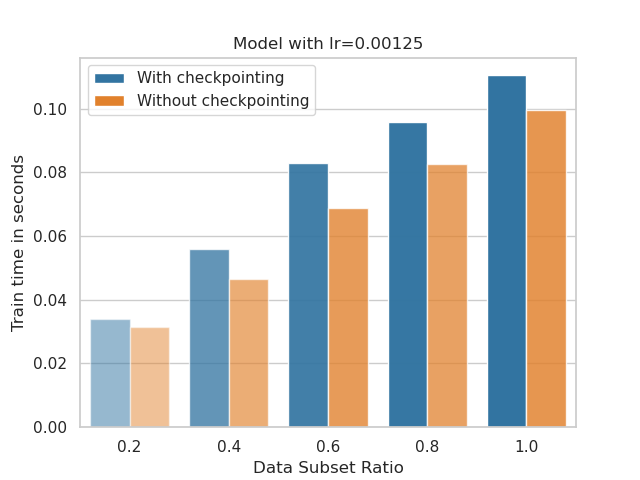
\includegraphics[width=\textwidth]{figures/22_07/iris/train_subset_0.00125.png}
        \caption{IRIS}
        \label{fig:11a}
    \end{subfigure}
    %\hfill
    \begin{subfigure}[b]{0.24\textwidth}
        \centering
        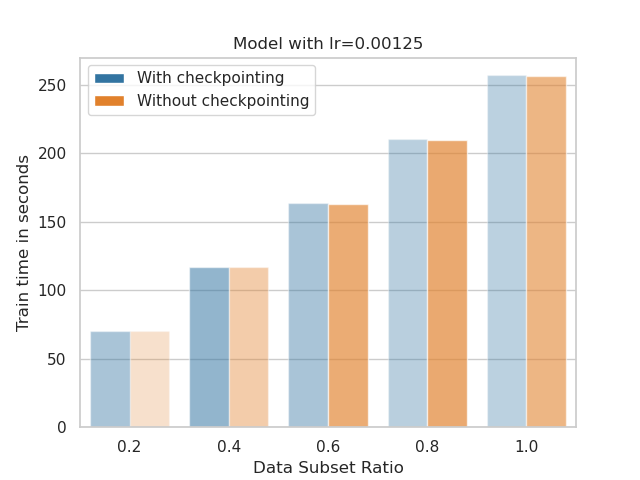
\includegraphics[width=\textwidth]{figures/22_07/10ep/train_subset_0.00125.png}
        \caption{MNIST 10 epochs}
        \label{fig:11b}
    \end{subfigure}
    %\hfill
    \begin{subfigure}[b]{0.24\textwidth}
        \centering
        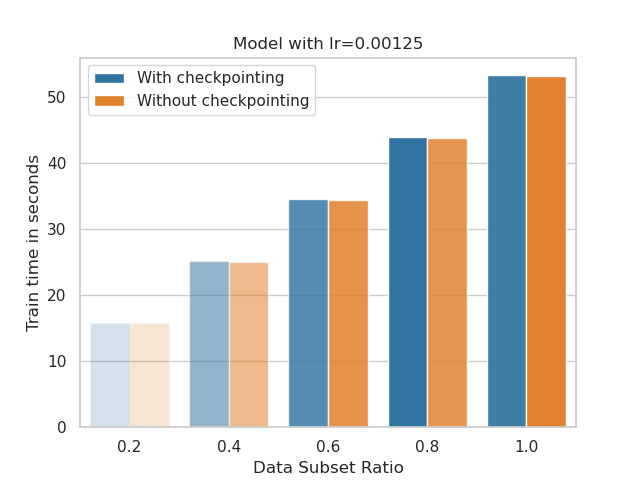
\includegraphics[width=\textwidth]{figures/22_07/2ep/train_subset_0.00125.png}
        \caption{MNIST 2 epochs}
        \label{fig:1111111111111111111111c}
    \end{subfigure}
    %\hfill
    \begin{subfigure}[b]{0.24\textwidth}
        \centering
        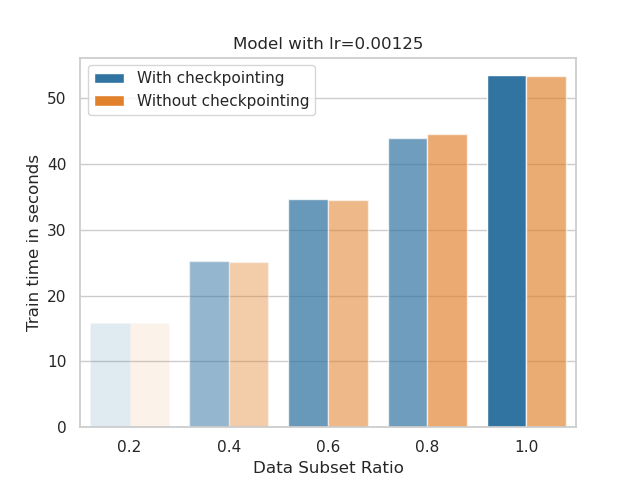
\includegraphics[width=\textwidth]{figures/22_07/2ep_smaller/train_subset_0.00125.png}
        \caption{MNIST 2 epochs, small model}
        \label{fig:11d}
    \end{subfigure}
    \caption{Visualization of the training time for every data subset ratio. A higher opacity means small validation performance difference to the optimum. An Adam optimizer and learning rate $1.25e^{-3}$ were used}
    \label{fig:11}
\end{figure}